\documentclass{article}

% Language setting
% Replace `english' with e.g. `spanish' to change the document language
\usepackage[english]{babel}
\usepackage[utf8]{inputenc}
\newcommand{\TF}{\operatorname{TF}}
\newcommand{\NRZ}{\operatorname{NRZ}}
\usepackage{stmaryrd}

\usepackage{float}

% Set page size and margins
% Replace `letterpaper' with `a4paper' for UK/EU standard size
\usepackage[a4paper,top=2cm,bottom=2cm,left=3cm,right=3cm,marginparwidth=1.75cm]{geometry}

% Useful packages
\usepackage{siunitx}
\usepackage{amsmath}
\usepackage{pgfplots}
\pgfplotsset{compat=newest}
\usetikzlibrary{plotmarks}
\usetikzlibrary{arrows.meta}
\usepgfplotslibrary{patchplots}
\usepackage{grffile}
\pgfplotsset{plot coordinates/math parser=false}
\newlength\figureheight
\newlength\figurewidth
  
\usepackage{graphicx}
\usepackage{hyperref}
%\newcommand{\TF}{\operatorname{TF}}
\newcommand{\sinc}{\operatorname{sinc}} 




\title{

\includegraphics[width=0.2\textwidth]{n7.png}
\\[1cm]
Project report -- Calcul scientifique

}
\author{Gautier Rancoule, Ewen Le Bihan}

\date{ENSEEIHT, département Sciences du Numérique}

\begin{document}

\maketitle

\setcounter{tocdepth}{3}
\tableofcontents

\section{Limitations of the power method}

We test with matrices of the following shapes

\begin{description}
    \item[1] $\begin{pmatrix} 1 & & & & (0) \\ & 2 & & & \\ & & 3 & & \\ & & & \ddots & \\ (0) & & & & n \end{pmatrix}$
    \item[2] $\operatorname{diag}(\verb|random(1e-10, 1)|)$
    \item[3] $\operatorname{diag}\left( (10^{5})^{- \frac{i-1}{n-1}} \right)_{i\in \llbracket 1, n \rrbracket} $
    \item[4] $\operatorname{diag}\left( 1 - (1 - 10^{-2}) \frac{i-1}{n-1} \right)_{i\in \llbracket 1, n \rrbracket} $
\end{description}

\begin{table}[H]
    \centering
    \label{tab:vitesse-algos}
    \begin{tabular}{c|cccc}
        Type / Alg & 1 & 2 & 3 & 4 \\\hline
        \verb|eig| (10) & $\SI{20}{ms}$ & $\SI{0}{ms}$ & $\SI{10}{ms}$ & $\SI{10}{ms}$ \\
        \verb|power| (11) & $\SI{1.77}{s}$ & $\SI{40}{ms}$ & $\SI{60}{ms}$ & $\SI{1.81}{s}$ \\
        \verb|power| (12) & $\SI{0.9}{s}$ & $\SI{60}{ms}$ & $\SI{60}{ms}$ & $\SI{0.93}{s}$ \\
        \verb|v0| (0) & 
    \end{tabular}
    \caption{Computation time comparisons}
\end{table}



\subsection{Main computing time drawback of the improved deflation method}


\verb|power_v12| is slower than \verb|power_v11| on matrices of type {\bf 2} (diagonal matrices of random floating point values close to zero).
It \emph{is} twice as fast on matrices of type {\bf 1} or {\bf 4}.

\section{Extending the power method to compute dominant eigenspace vectors}

\subsection{\verb|subspace_iter_v0|: a basic method to compute a dominant eigenspace}

Without orthonormalisation to force the vectors to evolve to different values during the iteration, there is a large chance that all output eigenvectors will be copies of one of the eigenvectors.

\subsubsection{Rayleigh quotient}

The size of $H$ is one order of magnitude less than $A$. Therefore, computing the spectral decompositon of $H$ is much less intensive than computing that of $A$'s.

\subsection{\verb|subspace_iter_v1|: improved version making use of Raleigh-Ritz projection}

\subsubsection{Convergence analysis step}


\begin{table}[H]
	\centering
	\caption{Steps of Algorithm 4}
	\label{tab:steps-alg-4}
	\begin{tabular}{l|l}
	Step & Code \\\hline
	Generate an initial set of $m$ orthogonal vectors & 48-49 \\
	$k=0$ & 38 \\
	$\text{PercentReached}=0$ & 40 \\
	$k=k+1$ 54 \\
	Compute  $Y$ such that $Y=A \cdot V$ & 56 \\
	$V \from \text{orthonormalization of the columns of $Y$}$ & 58 \\
	Rayleigh-Ritz project applied on matrix $A$ and $V$ & 61 \\
	Convergence analysis & 64-112 \\
	\end{tabular}
\end{table}

\section{\verb|subspace_iter_v2| and \verb|subspace_iter_v3|: towards an efficient solver}

\subsection{Block approach}

\paragraph{Question 8}

Let $n$ be the size of $A$ (such that $A \in \cM_{n, n}(\R)$). Computing $A^2$ takes $n^2(2n-1)$ flops.

Therefore, the computation is

\begin{align*}
	p n^2 (2n-1) \quad \text{flops}
\end{align*}

We have $V \in \cM_{n, m}(\R)$, therefore, computing $A^{p} \cdot V$ takes

\begin{align*}
	pn^2(2n-1) + nm(2n-1) &= (2n-1)n(pn+m) \quad \text{flops} \\
\end{align*}

By computing $A \cdot V$ first, then pre-multiplying the resulting \emph{vector} by $A$ $p-1$ times, most of the matrix products will be with a vector instead of between two matrices:

The cost is then

\begin{align*}
	nm(2n-1) + (p-1)nm(2n-1) &= pm(2n-1)  \quad \text{flops}
\end{align*}



\paragraph{Question 10}

\begin{table}[H]
	\centering
	\caption{Performance for a range of $p$ values}
	\label{tab:perf-p-values}
	\begin{tabular}{l|l}
		$p$ & # iterations \\\hline
		1  & 86   \\
		10 & 9  \\
		20 & 5  \\
		30 & 3  \\
		50 & 2  \\
		100 & 2  \\
		200 & \emph{does not converge} 
	\end{tabular}
\end{table}

By increasing the value of $p$, we do less orthonormalizations, and converge quicker to the result.

But, similarly to the \emph{learning rate} hyperparameter in neural networks, if we try to converge too quickly, finding a local minimum will never happen and we'll oscillate around, because the steps taken are too big.

\paragraph{Question 11}

We notice that some vectors converge faster to their eigenvector than others, specifically those that have a larger norm and those that are closer to the final guess. That faster convergence will allow for a greater eigenpair quality as the last steps of the convergence will be dedicated

\paragraph{Question 12}



\section{Numerical Experiments}

\paragraph{Question 14}

\begin{table}[H]
	\centering
	\begin{tabular}{cc}
		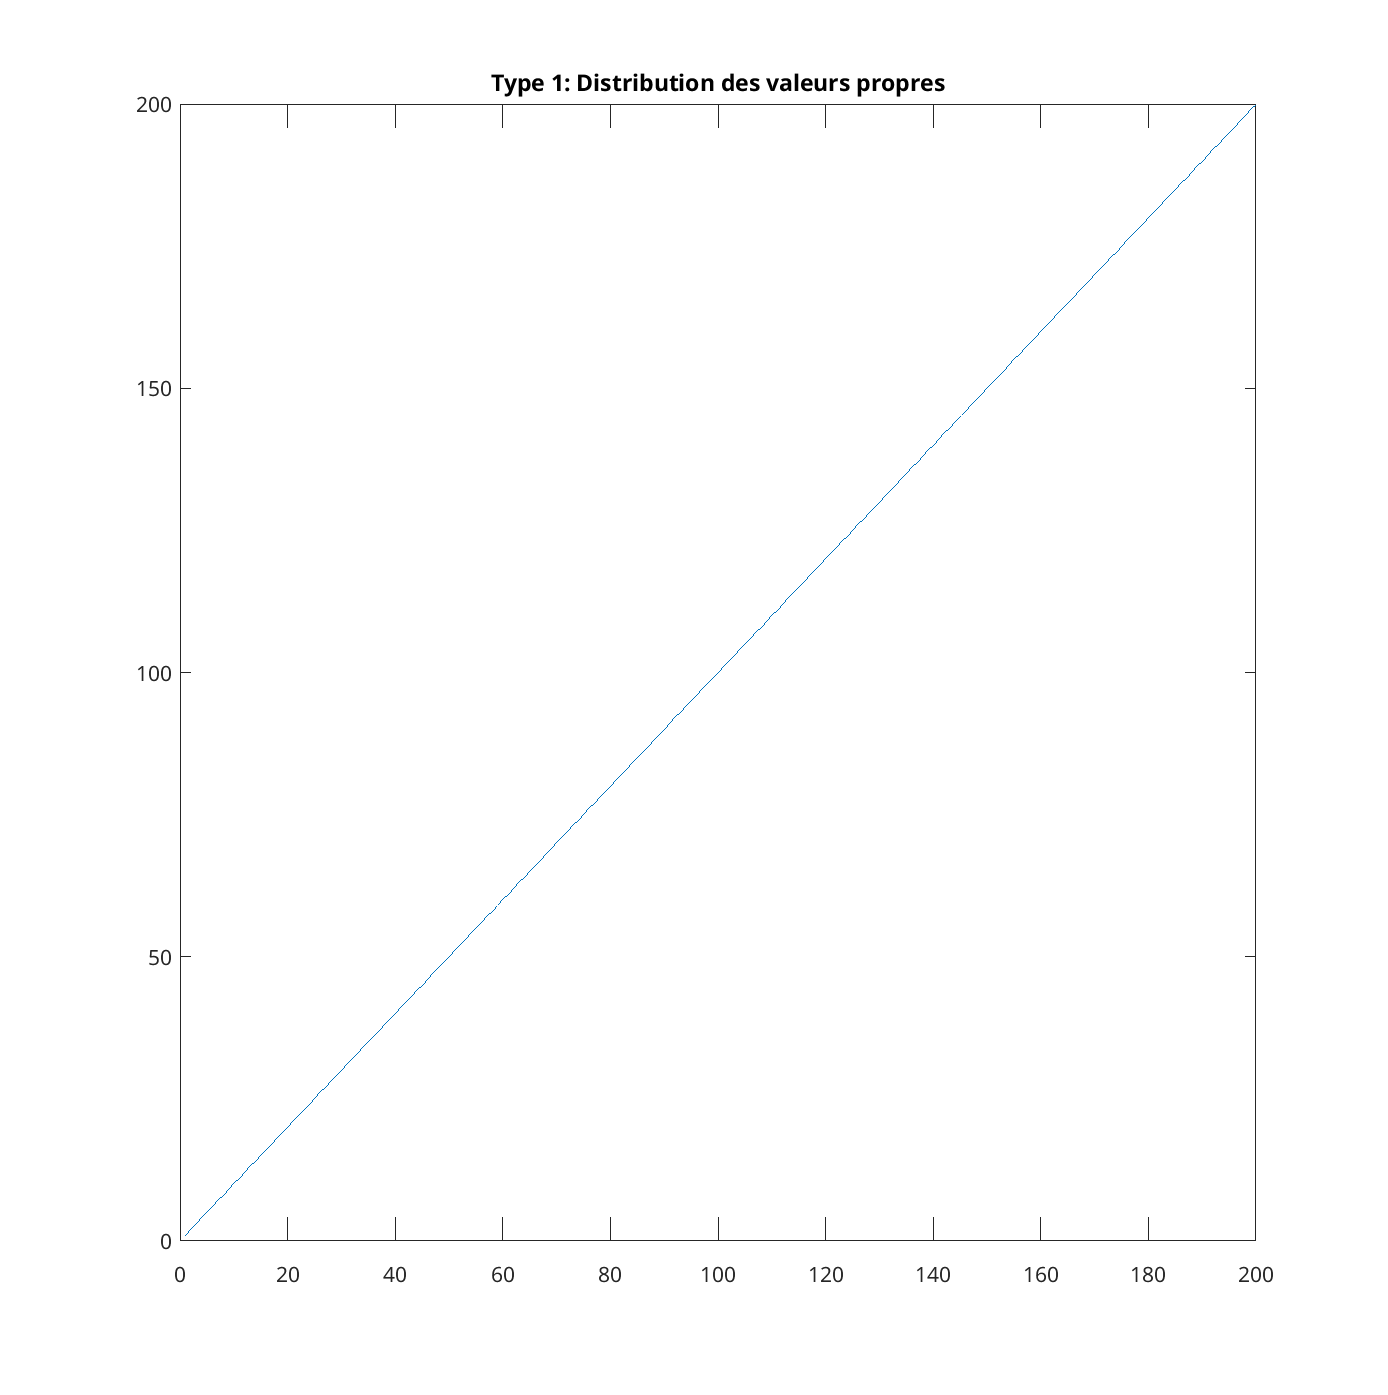
\includegraphics[width=0.3\textwidth]{distribution_type_1.png}
		& 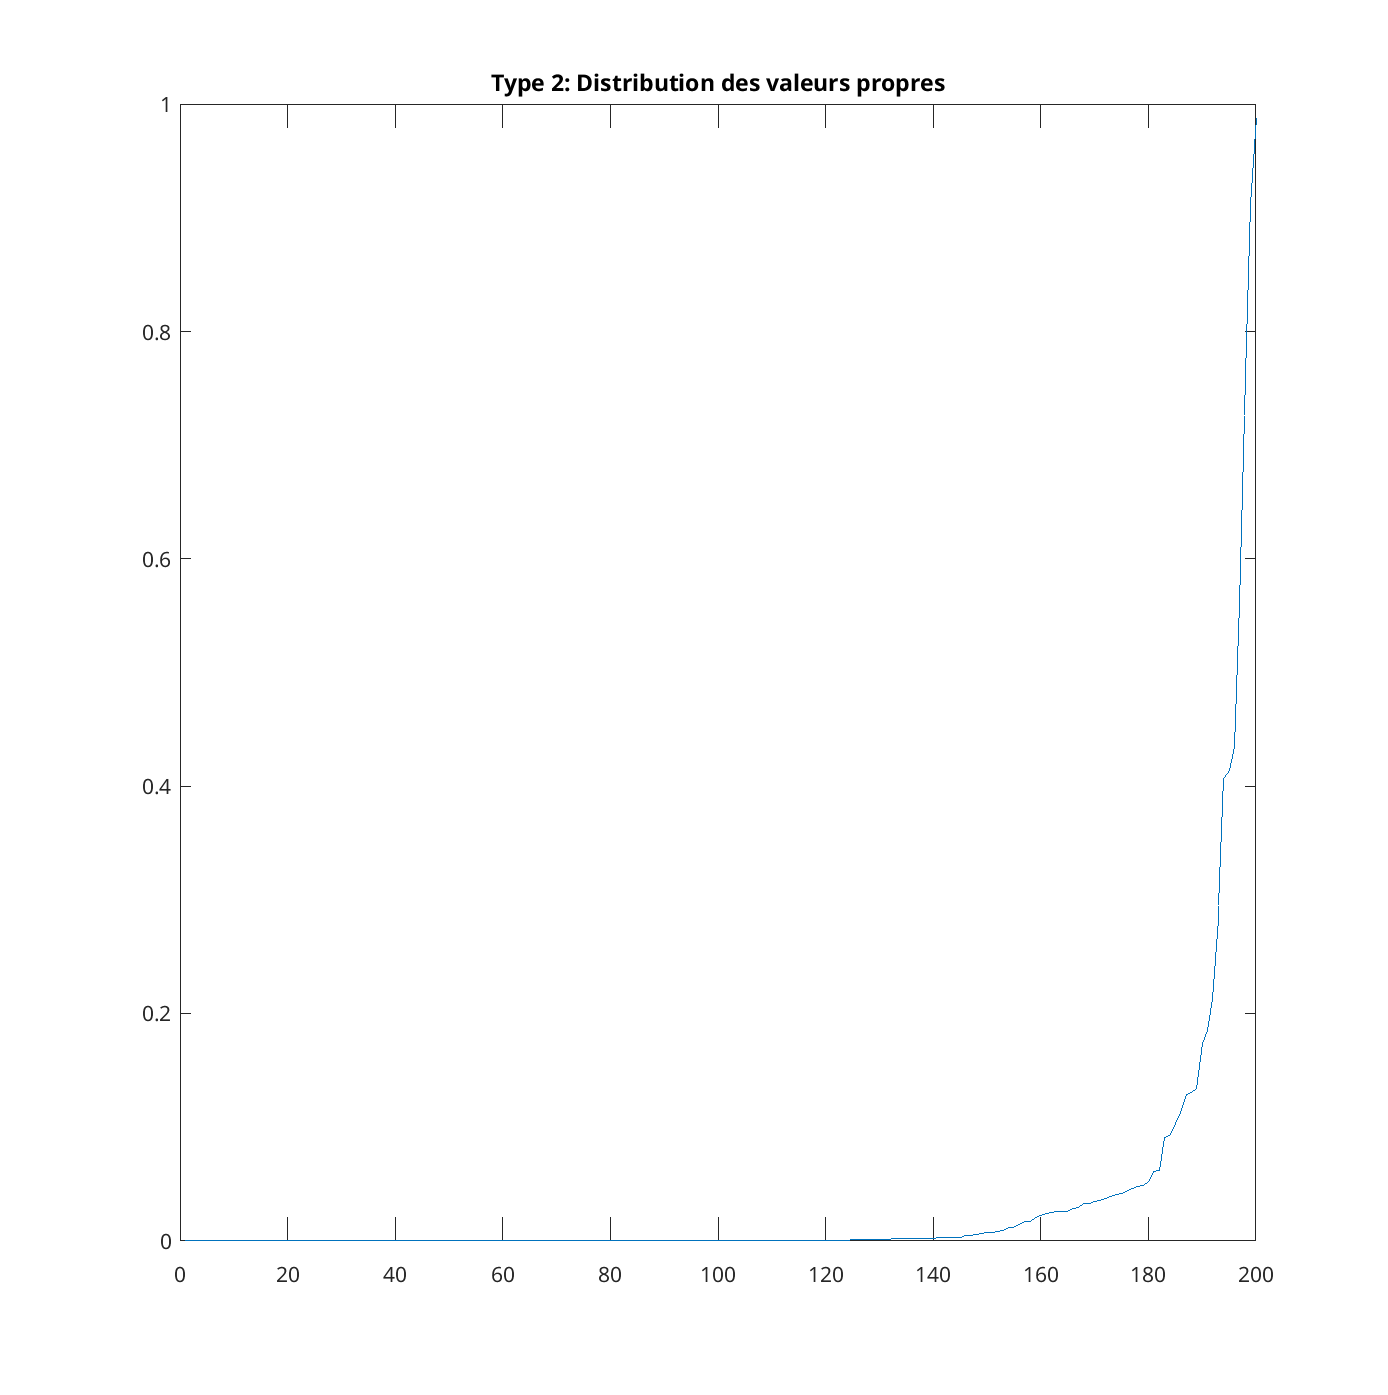
\includegraphics[width=0.3\textwidth]{distribution_type_2.png} \\
		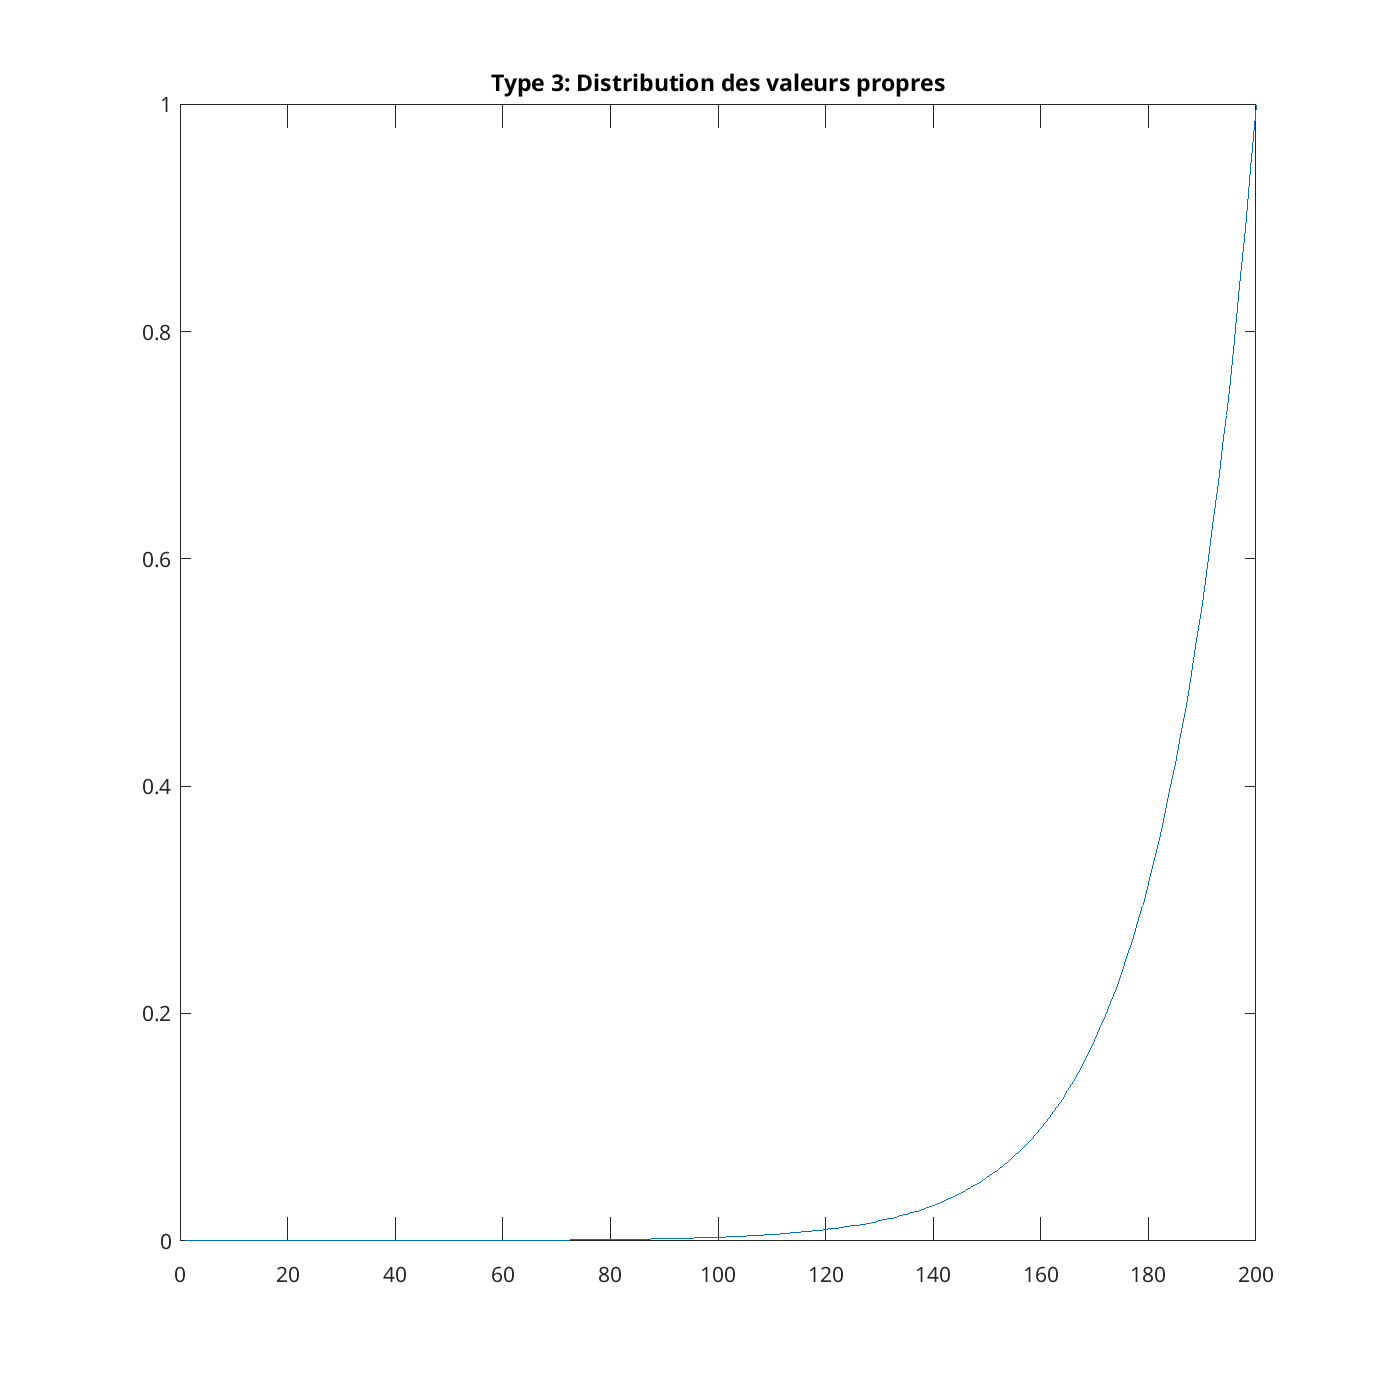
\includegraphics[width=0.3\textwidth]{distribution_type_3.png}
		& 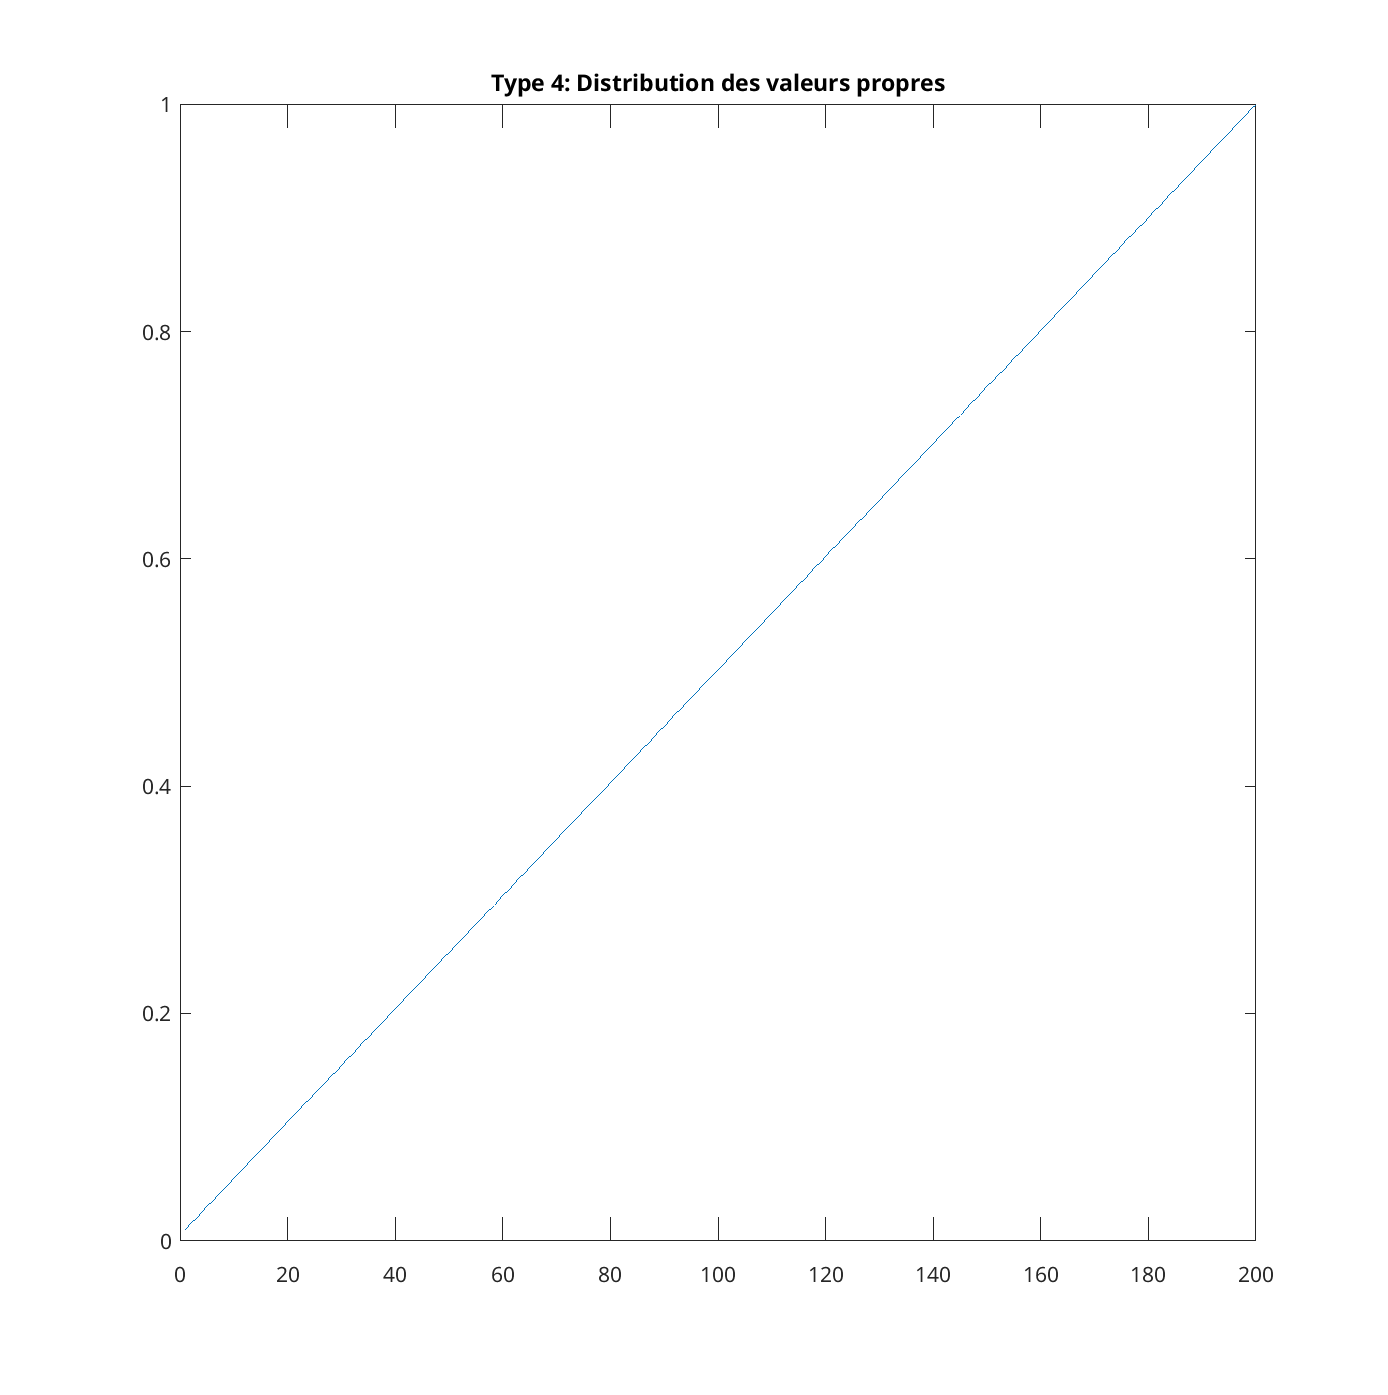
\includegraphics[width=0.3\textwidth]{distribution_type_4.png} \\
	\end{tabular}
\end{table}

\paragraph{Question 15}







\end{document}
